\documentclass[a4paper,12pt]{scrartcl}
\usepackage[utf8]{inputenc}
\usepackage[UKenglish]{isodate}
\usepackage{csquotes}
\usepackage{graphicx}
\usepackage{wrapfig}
\usepackage{enumitem}
\usepackage{pdflscape}
\usepackage[toc,page]{appendix}
\usepackage{geometry}
\usepackage{hyperref}
\usepackage{cleveref}
\usepackage{listings}
\usepackage{csvsimple}
\usepackage{booktabs}
\usepackage{longtable}
\usepackage{caption}
\usepackage{subcaption}
\usepackage[colorinlistoftodos]{todonotes}
\usepackage[british]{babel}
\usepackage{float}
%\usepackage[margin=1in]{geometry}
\usepackage{listings}
\usepackage{color}
 
\definecolor{codegreen}{rgb}{0,0.6,0}
\definecolor{codegray}{rgb}{0.5,0.5,0.5}
\definecolor{codepurple}{rgb}{0.58,0,0.82}
\definecolor{backcolour}{rgb}{0.95,0.95,0.92}
 
\lstdefinestyle{mystyle}{
	language=PHP,
    backgroundcolor=\color{backcolour},   
    commentstyle=\color{codegray},
    keywordstyle=\color{magenta},
    numberstyle=\tiny\color{codegray},
    stringstyle=\color{codegreen},
    basicstyle=\footnotesize,
    breakatwhitespace=false,         
    breaklines=true,                 
    captionpos=b,                    
    keepspaces=true,                 
    numbers=left,                    
    numbersep=5pt,                  
    showspaces=false,                
    showstringspaces=false,
    showtabs=false,                  
    tabsize=3,
    morekeywords={ new, __halt_compiler, abstract, and, array, as, break, callable, case, catch, class, clone, const, continue, declare, default, die, do, echo, else, elseif, empty, enddeclare, endfor, endforeach, endif, endswitch, endwhile, eval, exit, extends, final, for, foreach, function, global, goto, if, implements, include, include_once, instanceof, insteadof, interface, isset, list, namespace, new, or, print, private, protected, public, require, require_once, return, static, switch, throw, trait, try, unset, use, var, while, xor}
}

\lstset{language=Java,
  showspaces=false,
  showtabs=false,
  breaklines=true,
  showstringspaces=false,
  breakatwhitespace=true,
  commentstyle=\color{pgreen},
  keywordstyle=\color{pblue},
  stringstyle=\color{pred},
  basicstyle=\ttfamily,
  moredelim=[il][\textcolor{pgrey}]{$$},
  moredelim=[is][\textcolor{pgrey}]{\%\%}{\%\%}
}
 
\lstset{style=mystyle}

\graphicspath{ {images/} }
\usepackage[
	backend=biber,
	style=ieee,
	]{biblatex}

\addbibresource{references.bib}

\title{Case study of A National Programme for IT with regards to Managing Software Intensive Projects}
\author{James Fernando}
\date{\today}

\begin{document}
	
	\begin{titlepage}
		\maketitle
	\end{titlepage}
	
	\tableofcontents
	\newpage
	\section{Introduction}
	{
		
	}
	\section{Project Background}
	{
		NHS Connection for health is a section of the Department of Health which was in charge of producing a national programme for IT to allow for the sharing of patient information, this was set up in 2005\cite{nhsconnectingforhealth2019}. However some of the ideas for centralising patient information had been published in 1998. The quote below lists a couple of the ideas listed in a book published by the Department for Health in 1998.
		\begin{displayquote}{frankburns1998}
			\label{qoute:ConnectingForHealthPlans}
			individualised personal electronic records will be developed to provide NHS
			professionals with 24 hour secure access to the information important to
			individual patients’ care, when required. This will immeasurably improve
			emergency care and ensure any professional involved in the care of an
			individual is up to date with their treatment
			
			on-line services will be provided for GPs and their patients, to make hospital
			appointments as required or diagnostic results when due. The sight of hard
			pressed NHS professionals rummaging about in buff folders or hand-writing
			referrals and test requests will be consigned to history as soon as possible.
		\end{displayquote}
	}
	\section{Project Goal}
	{
		The national program for It was supposed to make use of technology to allow for easier and better sharing of patient information and medical information. Some of the systems and services has been listed below:
		\begin{displaycquote}{nhsconnectingforhealth2019}
			\begin{itemize}
				\item {creating an NHS Care Records Service to improve the sharing of patients' records across the NHS with their consent}
				\item {making it easier and faster for GPs and other primary care staff to choose and book hospital appointments for patients}
				\item {generating, transmitting and dispensing electronic prescriptions}
				\item {ensuring that the IT infrastructure can meet NHS needs now and in the future}
				\item {allowing x-rays and scans to be captured, viewed and stored digitally}
				\item {enabling patients' electronic health records to be transferred directly when they move from one GP practice to another}
				\item {linking the NHS with a secure email and directory service}
			\end{itemize}
		\end{displaycquote}
	}
	\section{Project Type}
	{
		\subsection{NTCP Diamond}
		{
			\begin{figure}
				\centering
				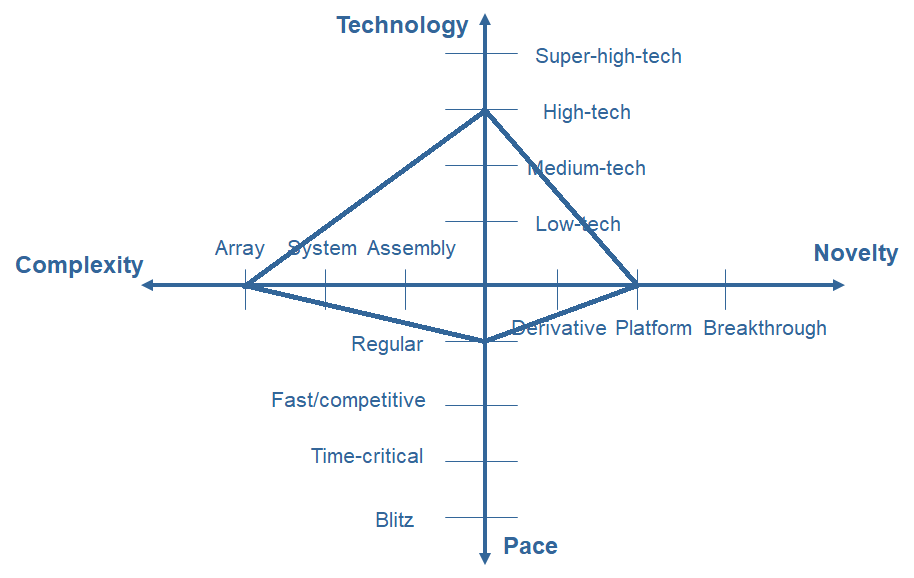
\includegraphics[width=\textwidth]{NationalProgrammeForITNTCP.png}
				\label{fig:NTCPDigram}
				\caption{Shows the NTCP Diamond created for the National Programme for IT project}
			\end{figure}
			\paragraph{Technology}
			{
				I've decided that the technological aspects are High tech this is due to the type of the project as it is a software project therefore will need to use the latests technologies and systems for it to run. also considering that this was launched in the early 2000's we should recognise that although it would probably be a medium tech project today the fact that software projects of this size would not have been though often back then, leads this to require a higher level of technology.
			}
			\paragraph{Novelty}
			{
				A software project of this size and complexity would very much have been the first of it's kind when it was first mentioned however a lot of the techniques and architecture would have been standard and commonplace. According to Taghreed Justinia it was \textquote{Deemed the world’s largest civil IT programme}\cite{Justinia2016}. 
			}
			\paragraph{Pace}
			{
				The National programme for IT was originally launched in 2002 and although I have not been able to find the original delivery dates it was dismantled in 2011 therefore showing that it was a very long term plan. Also due to the type of project it was the problem it was required for and the benefits it would provide would not change over time meaning this was not a time sensitive project with the only real limitation being the additional costs of taking more time.
			}
			\paragraph{Complexity}
			{
				The main reason why I have labelled this project as very complex is due to the size of the project the original aim was to provide a large number of services as a part of the project. Each of the services would have probably been considered a system on their own however due to the fact all of them have been merged I have labelled the project as a project of Array level complexity.
			}
		}
	}
	\section{Maturity Model}
	{
		
	}	
	\section{Appropriate and Inappropriate Approaches}
	{
		
	}
	\section{User Participation}
	{
		According to Dr Nowlan and Professor Hutton a major reason for the projects failure was due \textquote{clinicians were not taken into account and did not have sufficient say}\cite{Commons2007} this shows the lack of user/customer engagement in the project. It could be argued that this is because of the waterfall approach to product development which only really allows customer input at the beginning of the project whereas agile allows customer input throughout. I will get on to the software development methodologies in \cref{par:softwareDevelopmentMethodology}. The lack of user engagement is probably one of the reasons why the project is considered a failure especially as this is a good example of where user input could be used, as most hospitals and GP surgeries will have systems currently in place and understanding how clinicians use them and how they would like to use them would be a great input for the project. 
	}
	\section{Software Engineering}
	{
		\paragraph{Software Development Methodology}
		{
			\label{par:softwareDevelopmentMethodology}
			The National Programme for IT used a waterfall approach for software development\cite{Hoeksma2013}. I would describe this as a major failing in planning and decision making. Generally you would choose a waterfall methodology when your requirements are set in stone and changes to the deliverables of the project are very difficult to implement. In the case of the National Program for IT the requirements were provided at the start however due to the length of time the project covered they changed over the course of the project this also meant that different new technologies emerged which would have made developing the project easier. Also, although some parts of the programme was built on physical infrastructure this meant that some of the deliverables were unable to be changed the majority of the software would be changes easily as is the way with software products. It would have also made more sense to build the programme on top of the internet instead of using their own network as it would have been cheaper and reduce/remove the need for the external contracts and make it more suitable for an agile approach which tends to be cheaper and provide deliverables earlier and allow for more customer input. Hoeksma also goes on to say that \textquote{NHS England recently commissioned a replacement for the NHS “spine,” the data backbone built using the waterfall method. An agile developer quickly delivered a potential replacement for a tenth of the cost of the earlier system.}\cite{Hoeksma2013} which shows how much time and money could have been saved by using an agile methodology when implementing this project.
		}
	}
	\section{Integration with Current Systems}
	{
		One of the requirements for the project was for the local trusts to implement their own system to transfer the current patient information to the new National Programme for IT system. The National Programme for IT Implementation Guide\cite{HealthImplementationGuidanceteam2007} gives an overview of how the systems should be implemented and suggests that software should be developed using national standards.
	}
	\section{Conclusion}
	{

	}
	
	
	\newpage
	
	\printbibliography[heading=bibintoc,title=References]
\end{document}
